\section{Hardware design}
\vspace{-0.5cm}
Til projektet er der købt mange færdige hardware moduler. Switch boardet er det eneste hardware der er blevet designet. 

\vspace{-0.3cm}

\subsection{Switch board}
\vspace{-0.4cm}
I dette afsnit beskrives hardware designet af switch boardet. Boardet er designet så det kan switche mellem manuel og autonom flyvning. Når der flyves manuelt lader switch boardet styringssignaler fra remote controller styre dronen og når der flyves autonomt er det signaler fra main controller der styrer dronen.

På figur \ref{fig:switchboard_design} vises designet af switch boardet.
Styringssignaler fra main controller og remote controller sendes begge til switch boardet, hvor de sendes ind i 2-input AND gates. AND gates på højre side håndterer signaler fra remote controller og på venstre side håndteres signaler fra main controller. Hvilket output der kommer på de forskellige AND gates afhænger af signalet der sendes ind på kontrol pin. Outputtet fra AND gates med samme styringssignal (fx. Throttle) sendes til OR gates, som sender det rette styringssignal videre til flight control boardet. 


\begin{figure}[H]
	\centering
	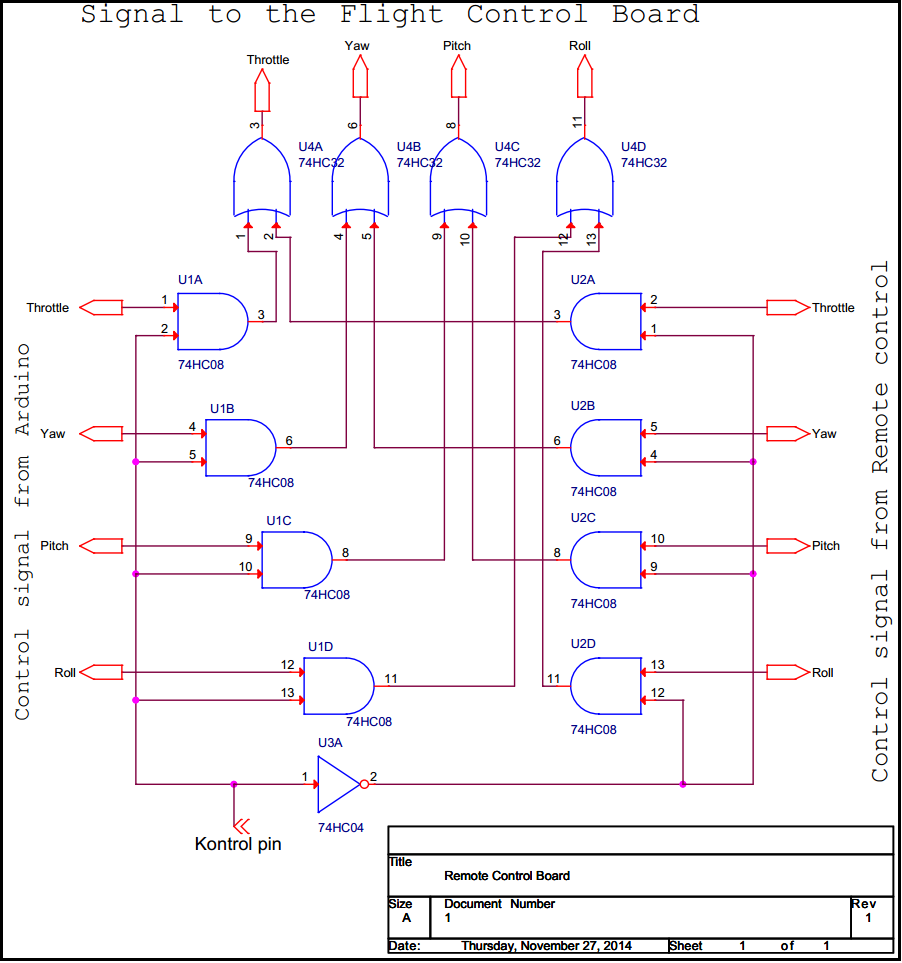
\includegraphics[width=0.87\textwidth]{Billeder/hardware/switch_board_diagram.png}
	\caption{Switch board design}
	\label{fig:switchboard_design}
\end{figure}

\newpage

\subsection{}
I dette afsnit beskrives hvordan systemets forskellige hardware dele sammensættes.
Først i afsnittet vises en stykliste der beskriver systemets hardware dele, dernæst vises hvordan hardware delene er koblet sammen.

\textbf{Stykliste}\\
3G/GPS module\\
Ultralydssensor\\
Main controller\\
Flight control board\\
Fjernbetjening + Receiver\\
Switch board\\

De fem første moduler er færdigkøbte hardware moduler, kun switch boardet er designet og implementeret af gruppen. Til konstruktion af switch boardet er der brugt: To AND gates af typen 74HC08, en OR gate af typen 74HC32 og en INVERTER af typen 74HC04.


\begin{figure}[H]
	\centering
	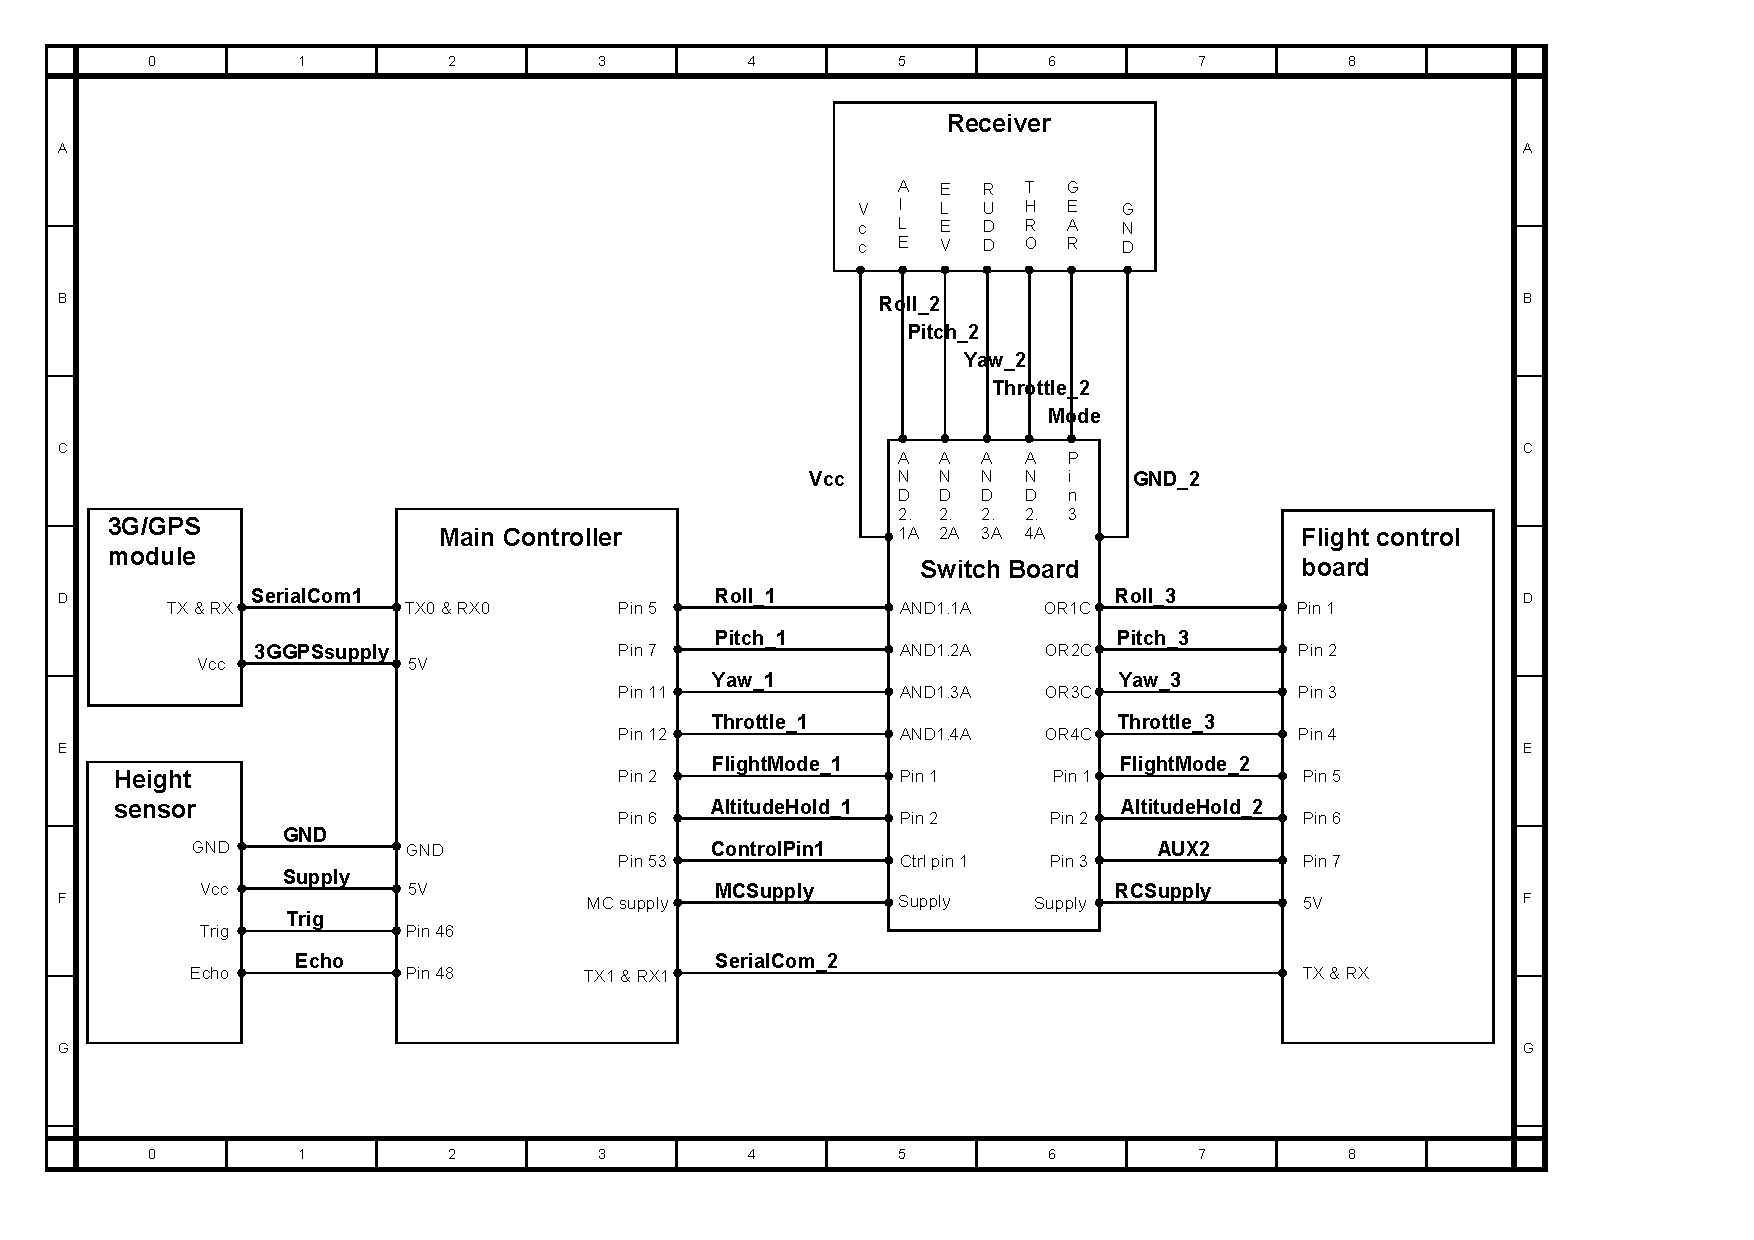
\includegraphics[width=1\textwidth]{Billeder/hardware/hardware_oversigt.png}
	\caption{Switch board design}
	\label{fig:switchboard_design}
\end{figure}
